\documentclass[fancy, oneside, mastersfancy, ms]{byuthesis}
\usepackage{bookmark}


\usepackage{color}
\usepackage{fancyvrb}
\newcommand{\VerbBar}{|}
\newcommand{\VERB}{\Verb[commandchars=\\\{\}]}
\DefineVerbatimEnvironment{Highlighting}{Verbatim}{commandchars=\\\{\}}
% Add ',fontsize=\small' for more characters per line
\usepackage{framed}
\definecolor{shadecolor}{RGB}{241,243,245}
\newenvironment{Shaded}{\begin{snugshade}}{\end{snugshade}}
\newcommand{\AlertTok}[1]{\textcolor[rgb]{0.68,0.00,0.00}{#1}}
\newcommand{\AnnotationTok}[1]{\textcolor[rgb]{0.37,0.37,0.37}{#1}}
\newcommand{\AttributeTok}[1]{\textcolor[rgb]{0.40,0.45,0.13}{#1}}
\newcommand{\BaseNTok}[1]{\textcolor[rgb]{0.68,0.00,0.00}{#1}}
\newcommand{\BuiltInTok}[1]{\textcolor[rgb]{0.00,0.23,0.31}{#1}}
\newcommand{\CharTok}[1]{\textcolor[rgb]{0.13,0.47,0.30}{#1}}
\newcommand{\CommentTok}[1]{\textcolor[rgb]{0.37,0.37,0.37}{#1}}
\newcommand{\CommentVarTok}[1]{\textcolor[rgb]{0.37,0.37,0.37}{\textit{#1}}}
\newcommand{\ConstantTok}[1]{\textcolor[rgb]{0.56,0.35,0.01}{#1}}
\newcommand{\ControlFlowTok}[1]{\textcolor[rgb]{0.00,0.23,0.31}{#1}}
\newcommand{\DataTypeTok}[1]{\textcolor[rgb]{0.68,0.00,0.00}{#1}}
\newcommand{\DecValTok}[1]{\textcolor[rgb]{0.68,0.00,0.00}{#1}}
\newcommand{\DocumentationTok}[1]{\textcolor[rgb]{0.37,0.37,0.37}{\textit{#1}}}
\newcommand{\ErrorTok}[1]{\textcolor[rgb]{0.68,0.00,0.00}{#1}}
\newcommand{\ExtensionTok}[1]{\textcolor[rgb]{0.00,0.23,0.31}{#1}}
\newcommand{\FloatTok}[1]{\textcolor[rgb]{0.68,0.00,0.00}{#1}}
\newcommand{\FunctionTok}[1]{\textcolor[rgb]{0.28,0.35,0.67}{#1}}
\newcommand{\ImportTok}[1]{\textcolor[rgb]{0.00,0.46,0.62}{#1}}
\newcommand{\InformationTok}[1]{\textcolor[rgb]{0.37,0.37,0.37}{#1}}
\newcommand{\KeywordTok}[1]{\textcolor[rgb]{0.00,0.23,0.31}{#1}}
\newcommand{\NormalTok}[1]{\textcolor[rgb]{0.00,0.23,0.31}{#1}}
\newcommand{\OperatorTok}[1]{\textcolor[rgb]{0.37,0.37,0.37}{#1}}
\newcommand{\OtherTok}[1]{\textcolor[rgb]{0.00,0.23,0.31}{#1}}
\newcommand{\PreprocessorTok}[1]{\textcolor[rgb]{0.68,0.00,0.00}{#1}}
\newcommand{\RegionMarkerTok}[1]{\textcolor[rgb]{0.00,0.23,0.31}{#1}}
\newcommand{\SpecialCharTok}[1]{\textcolor[rgb]{0.37,0.37,0.37}{#1}}
\newcommand{\SpecialStringTok}[1]{\textcolor[rgb]{0.13,0.47,0.30}{#1}}
\newcommand{\StringTok}[1]{\textcolor[rgb]{0.13,0.47,0.30}{#1}}
\newcommand{\VariableTok}[1]{\textcolor[rgb]{0.07,0.07,0.07}{#1}}
\newcommand{\VerbatimStringTok}[1]{\textcolor[rgb]{0.13,0.47,0.30}{#1}}
\newcommand{\WarningTok}[1]{\textcolor[rgb]{0.37,0.37,0.37}{\textit{#1}}}

\providecommand{\tightlist}{%
  \setlength{\itemsep}{0pt}\setlength{\parskip}{0pt}}\usepackage{longtable,booktabs,array}
\usepackage{calc} % for calculating minipage widths
% Correct order of tables after \paragraph or \subparagraph
\usepackage{etoolbox}
\makeatletter
\patchcmd\longtable{\par}{\if@noskipsec\mbox{}\fi\par}{}{}
\makeatother
% Allow footnotes in longtable head/foot
\IfFileExists{footnotehyper.sty}{\usepackage{footnotehyper}}{\usepackage{footnote}}
\makesavenoteenv{longtable}
\usepackage{graphicx}
\makeatletter
\def\maxwidth{\ifdim\Gin@nat@width>\linewidth\linewidth\else\Gin@nat@width\fi}
\def\maxheight{\ifdim\Gin@nat@height>\textheight\textheight\else\Gin@nat@height\fi}
\makeatother
% Scale images if necessary, so that they will not overflow the page
% margins by default, and it is still possible to overwrite the defaults
% using explicit options in \includegraphics[width, height, ...]{}
\setkeys{Gin}{width=\maxwidth,height=\maxheight,keepaspectratio}
% Set default figure placement to htbp
\makeatletter
\def\fps@figure{htbp}
\makeatother
\newlength{\cslhangindent}
\setlength{\cslhangindent}{1.5em}
\newlength{\csllabelwidth}
\setlength{\csllabelwidth}{3em}
\newlength{\cslentryspacingunit} % times entry-spacing
\setlength{\cslentryspacingunit}{\parskip}
\newenvironment{CSLReferences}[2] % #1 hanging-ident, #2 entry spacing
 {% don't indent paragraphs
  \setlength{\parindent}{0pt}
  % turn on hanging indent if param 1 is 1
  \ifodd #1
  \let\oldpar\par
  \def\par{\hangindent=\cslhangindent\oldpar}
  \fi
  % set entry spacing
  \setlength{\parskip}{#2\cslentryspacingunit}
 }%
 {}
\usepackage{calc}
\newcommand{\CSLBlock}[1]{#1\hfill\break}
\newcommand{\CSLLeftMargin}[1]{\parbox[t]{\csllabelwidth}{#1}}
\newcommand{\CSLRightInline}[1]{\parbox[t]{\linewidth - \csllabelwidth}{#1}\break}
\newcommand{\CSLIndent}[1]{\hspace{\cslhangindent}#1}

\usepackage{booktabs}
\usepackage{longtable}
\usepackage{array}
\usepackage{multirow}
\usepackage{wrapfig}
\usepackage{float}
\usepackage{colortbl}
\usepackage{pdflscape}
\usepackage{tabu}
\usepackage{threeparttable}
\usepackage{threeparttablex}
\usepackage[normalem]{ulem}
\usepackage{makecell}
\usepackage{xcolor}
\usepackage{siunitx}
\usepackage{booktabs}
\usepackage{longtable}
\usepackage{array}
\usepackage{multirow}
\usepackage{wrapfig}
\usepackage{float}
\usepackage{colortbl}
\usepackage{pdflscape}
\usepackage{tabu}
\usepackage{threeparttable}
\usepackage{threeparttablex}
\usepackage[normalem]{ulem}
\usepackage[utf8]{inputenc}
\usepackage{makecell}
\usepackage{xcolor}
\makeatletter
\makeatother
\makeatletter
\@ifpackageloaded{bookmark}{}{\usepackage{bookmark}}
\makeatother
\makeatletter
\@ifpackageloaded{caption}{}{\usepackage{caption}}
\AtBeginDocument{%
\ifdefined\contentsname
  \renewcommand*\contentsname{Table of contents}
\else
  \newcommand\contentsname{Table of contents}
\fi
\ifdefined\listfigurename
  \renewcommand*\listfigurename{List of Figures}
\else
  \newcommand\listfigurename{List of Figures}
\fi
\ifdefined\listtablename
  \renewcommand*\listtablename{List of Tables}
\else
  \newcommand\listtablename{List of Tables}
\fi
\ifdefined\figurename
  \renewcommand*\figurename{Figure}
\else
  \newcommand\figurename{Figure}
\fi
\ifdefined\tablename
  \renewcommand*\tablename{Table}
\else
  \newcommand\tablename{Table}
\fi
}
\@ifpackageloaded{float}{}{\usepackage{float}}
\floatstyle{ruled}
\@ifundefined{c@chapter}{\newfloat{codelisting}{h}{lop}}{\newfloat{codelisting}{h}{lop}[chapter]}
\floatname{codelisting}{Listing}
\newcommand*\listoflistings{\listof{codelisting}{List of Listings}}
\makeatother
\makeatletter
\@ifpackageloaded{caption}{}{\usepackage{caption}}
\@ifpackageloaded{subcaption}{}{\usepackage{subcaption}}
\makeatother
\makeatletter
\@ifpackageloaded{tcolorbox}{}{\usepackage[skins,breakable]{tcolorbox}}
\makeatother
\makeatletter
\@ifundefined{shadecolor}{\definecolor{shadecolor}{rgb}{.97, .97, .97}}
\makeatother
\makeatletter
\makeatother
\makeatletter
\makeatother

\title{Simulating Incident Management Team Response and Performance}
\author{Daniel Jarvis}

% On the custom title page, use the same title, but format as you like
\customtitle{Simulating Incident Management Team Response and
Performance}

% This is the date of graduation
\date{2023-06-25}

% If your degree is not a PhD or MS, then you can overwrite the degree using 
% the \degree command: \degree{Bachelors of Basics}

% Your department
\department{Civil and Construction Engineering}

% The names of your committee members
\committeechair{Gregory S. Macfarlane}
  \committeemember{Grant G. Schultz}
  \committeemember{Gustavious P. Williams}

\keywords{
    Incident Management Teams; Incident Simulation;  
    Transportation Modeling
}

\begin{document}

\frontmatter
\titlepage
\cleardoublepage

\customtitlepage
\cleardoublepage


  \begin{abstract}
The effectiveness of Incident Management Teams (IMT) in reducing the
duration and impact of traffic incidents is well-documented. The
capacity of large-scale simulation models to illustrate the negative
effects of these incidents on vehicle delays and excess user costs (EUC)
is also widely recognized. However, there is a gap in research
integrating large-scale simulation modeling with IMT performance
analysis. This study uses the Multi-Agent Transport Simulation (MATSim)
to assess how incidents and IMT influence Utah's Wasatch Front regional
network and evaluates their performance under hypothetical scenarios.

Our findings validate the role of IMT in decreasing delays and EUC. The
simulation investigates the potential effects of increased incident
frequency and IMT expansion, revealing that more incidents increase
delays, whereas more IMT units can mitigate these effects and improve
response times.

The MATSim model we developed demonstrates the potential of dynamic
large-scale modeling to evaluate incident management strategies in ways
that previous studies did not. This model could serve as a valuable tool
for further evaluating the performance of Utah's IMT program, with the
potential to offer new perspectives on optimizing team deployment and
scheduling efficiency.
\end{abstract}
\cleardoublepage

\begin{acknowledgments}
I want to extend my gratitude to the Utah Department of Transportation
for their substantial financial backing, which was essential for the
completion of my research and thesis project. I am equally grateful to
the technical advisory committee, whose expert guidance and invaluable
feedback were critical throughout my research endeavor. Their in-depth
understanding of Utah's traffic incident management programs was a
crucial contributor to the successful outcome of this study.

My sincere thanks are extended to my fellow research assistants at
BYU---Joel Hyer, Harrison Holdsworth, and Brynn Woolley. Joel's
insightful analysis and the vital data he provided from the IMT
Performance Phase III project were indispensable. Harrison's
wide-ranging input, from his diligent compilation of research on IMT
optimization to his collaborative efforts in drafting the literature
review, proved instrumental. His ability to seamlessly connect Joel's
work with my research was invaluable. Brynn's expertise in developing
the transportation model, her astute analysis of its findings, and her
assistance in refining and editing this report added significantly to
the quality of my work.

Profound appreciation is due to my faculty advisors and the members of
my thesis committee, Drs. Macfarlane, Schultz, and Williams, for their
unwavering support. I am particularly indebted to Dr.~Macfarlane for his
exceptional mentorship as an advisor, educator, and friend. His
patience, wisdom, and encouragement have been instrumental at every
stage of my academic journey. His faith in me and consistent support
have been the pillars of my personal development and the achievements of
this research.

Lastly, I offer thanks to my parents, Duane and Jodi Jarvis, for their
steadfast encouragement and belief in me throughout my academic
pursuits. Their encouragement and reassurance have been a source of
immense strength, especially during this significant stage of my life. I
am forever grateful for the stability and unwavering support they have
so selflessly provided.
\end{acknowledgments}
\cleardoublepage

	\tableofcontents*
	\cleardoublepage

	\listoffigures
	\cleardoublepage

	\listoftables
	\cleardoublepage

\mainmatter
\bookmarksetup{startatroot}

\hypertarget{introduction}{%
\chapter{Introduction}\label{introduction}}

\footnote{This is a draft of a manuscript, authored by Jarvis,
  Macfarlane, Woolley, and Schultz. It is prepared for submission to the
  Transportation Research Board. Any use of the pronoun `we' throughout
  this document refers collectively to the research team, all of whom
  will be listed as authors upon the manuscript's publication as an
  article.}Incident Management Teams (IMT) are service vehicles that
collaborate with highway patrol units to manage traffic after an
incident and provide timely roadside assistance. They are strategically
important for improving highway operations, particularly during peak
traffic times, helping to effectively alleviate congestion and
associated user costs. Capable of quickly addressing a range of
incidents from minor vehicle breakdowns to severe multi-car collisions,
IMT are crucial in controlling traffic and restoring normal flow on the
roadways.

States like Utah have long benefited from IMT, witnessing notable
reductions in congestion and traffic-related costs (Bennett, 2021). The
effectiveness of IMT, influenced by factors such as response times
(Schultz et al., 2019), fleet size (Kim et al., 2012), and deployment
locations (Ozbay et al., 2013), is well-documented. However, the current
understanding primarily stems from ad-hoc models and independent
initiatives, leaving a gap in regional-scale traffic delay modeling
associated with incident management.

A study conducted by Kaddoura \& Nagel (2018) highlights the potential
of large-scale traffic models to assess the regional impact of
incidents, demonstrating that such incidents can significantly increase
congestion and average vehicle travel times within a simulated network.
However, their model does not evaluate the impact of IMT strategies.
This research aims to address this limitation by merging insights on IMT
effectiveness with a large-scale regional traffic model. This approach
is designed to underscore the impacts of traffic incidents and IMT
interventions within a simulated network.

In this research, we present a model of IMT response to incidents on
freeways in the Wasatch Front region of Utah. The model uses the Multi
Agent Transportation Simulation (MATSim) to evaluate IMT effectiveness
within various traffic incident scenarios. After conducting 60
simulations, we compared their outcomes and evaluated the effectiveness
of IMT at improving traffic conditions and reducing congestion.

We used the Multi Agent Transportation Simulation (MATSim) to model
model roadway conditions along the Wasatch Front region of Utah. The
model was used to evaluate IMT effectiveness within various traffic
incident scenarios. After conducting 60 simulations, we compared their
outcomes and evaluated the effectiveness of IMT at improving traffic
conditions and reducing congestion.

The paper proceeds in a typical order.
\protect\hyperlink{sec-literature}{The literature review} contains a
discussion of previous research into IMT effectiveness and optimization.
\protect\hyperlink{sec-methods}{A methodology section} describes the
simulation and scenario construction, while
\protect\hyperlink{sec-results}{the results} present the findings of the
analysis alongside a discussion of their implications. The paper
\protect\hyperlink{sec-conclusions}{conclusions section} provides an
outline of future research motivated by this study's limitations.

\bookmarksetup{startatroot}

\hypertarget{sec-literature}{%
\chapter{Literature Review}\label{sec-literature}}

Traffic incident management in general --- and IMT in particular --- are
not strictly new innovations. The Federal Highway Administration (FHWA)
publishes the \emph{Traffic Incident Management Handbook} (FHWA, 2000),
which defines traffic incident management as:

\begin{quote}
\emph{The systematic, planned, and coordinated use of human,
institutional, mechanical, and technical resources to reduce the
duration and impact of incidents and improve the safety of motorists,
crash victims, and incident responders. (p.~1-1)}
\end{quote}

The handbook details the process of how to implement a traffic incident
management program as well as improve it. The manual covers various
aspects of incident management, including the responsibilities of
emergency medical teams, law enforcement, and other responding entities.
For this research, we focus on the dedicated traffic incident management
teams operated by departments of transportation or similar agencies and
not on other types of first responders.

FHWA has established performance measures to develop a framework to
quantify improvements to IMT operations (FHWA, 2000). A specific measure
related to this research is roadway clearance time (RCT): the time
between the first recordable awareness of the incident and the time all
lanes open for traffic flow. Numerous studies have assessed the impact
of Traffic Incident Management programs on traffic conditions, utilizing
the performance measures provided by FHWA. A particularly noteworthy
study conducted by Schultz et al. (2019) explores the relationship
between IMT response time (RT) and RCT. This research leveraged
interconnected data from the Utah Department of Transportation (UDOT)
and the Utah Highway Patrol (UHP), aiming to quantify the traffic
improvements resulting from swift IMT interventions at incident sites.
Analyzing 121 incidents, the study found that a one-minute delay in IMT
response correlated with a 0.8-minute increase in RCT. This delay also
impacted an additional 93 vehicles, added roughly 34.6 minutes to the
network's total estimated travel time, and resulted in an extra \$925 in
excess user costs (ECU). Schultz et al. (2019) established a clear
connection between timely IMT responses and improved traffic conditions,
underscoring the importance of rapid intervention.

Skabardonis et al. (1998) confirmed the effectiveness of IMT in their
study, concluding that IMT in California effectively reduced incident RT
and ECU. Skabardonis et al. (1998) found that, on average, total
incident RT was 15 minutes longer when California Highway Patrol (CHP)
responded without the support of IMT. Using a system to assign a cost
per traveler per unit of time to vehicles in the observed area, the
authors determined that IMT units had a cost-to-benefit ratio of 5:1.
They also concluded that CHP officers spent less time on incidents
(including vehicle breakdowns) when assisted by IMT services.

\hypertarget{sec-lit_imt_opt}{%
\section{IMT Optimization}\label{sec-lit_imt_opt}}

Given the evidence that IMT programs improve traffic conditions and
reduce costs for government entities and individuals, it becomes crucial
to further research avenues to maximize these benefits. One possible
strategy is the strategic placement of IMT units, optimizing their
spatial effectiveness to enhance their impact. Enhancing IMT programs
often focuses on the precise deployment of individual trucks and the
strategic positioning of IMT depots---locations where inactive trucks
await dispatch. For scenarios where IMT vehicles are actively on patrol,
research often concerns designing an efficient service area. Various
methodologies have been applied to tackle this allocation challenge.
While some studies employ statistical models, incorporating a range of
variables to maximize specific performance measures, others opt for
digital modeling as a solution.

For instance, Ozbay et al. (2013) designed a mixed-integer programming
model with probabilistic constraints to optimize the allocation of IMT
across ``depots'' or staging areas in New Jersey. This innovative
approach, grounded in known probabilities of various incident types,
strategically positions IMT units to respond to incidents, taking into
account future probabilities on the network. The primary goals were to
minimize incident management costs and maximize the likelihood that
every incident receive assistance. The model was applied to a simplified
South Jersey Highway network, utilizing traffic incident data from the
region to inform demand distribution. Through this application, an
optimal number of depots and truck assignments were determined. However,
the lack of a comparative analysis with pre-existing depot and unit
distributions meant that the exact improvements yielded by the model
remained unquantified.

Where Ozbay et al. (2013) focused on optimizing the IMT allocation in
specific zones, others have researched their effectiveness as roaming
entities. Lou et al. (2011) developed a mixed-integer nonlinear
optimization model and proposed different algorithms to minimize the RT
of IMT. They modeled IMT within specific freeway sections, and incident
frequencies were generated randomly on the network, given the mean and
standard deviations of incident occurrence on each link in the network.
The study focused on developing and optimizing these algorithms for
broad implementation rather than focusing on any particular network or
reducing response times in specific areas. They implemented a template
Sioux Falls network into the model as a practical demonstration.
Compared to the existing deployment plan in Sioux Falls, the
algorithm-generated plans could potentially reduce total RT by
16.5-20.8\%.

Each of the studies mentioned attempts to understand optimal IMT
deployment based on ad-hoc models, specially constructed utility
functions, or similar stand-alone efforts. While their results provide
valuable insights, they might be limited in their scope, as they do not
explicitly attempt to model the traffic delay associated with incident
management at a large scale. Research modeling the effects of incidents
on region-scale traffic networks is a recent innovation, providing a
more holistic view of the impact. This approach is potentially
beneficial for comprehensively assessing the effectiveness of IMT and
paves the way for our subsequent discussion on Incident Modeling, where
we will discuss the advancements and applications of this innovative
research domain.

\hypertarget{sec-inc_modeling}{%
\section{Incident Modeling}\label{sec-inc_modeling}}

The majority of traffic models utilized to study the impacts of
incidents and incident management are Dynamic Traffic Assignment (DTA)
models. These models demonstrate how congestion and travel times
fluctuate over time, varying for different vehicles (Boyles, 2018).
Their capability to represent variance over time make DTA models
particularly advantageous for depicting the unpredictability of
incidents. A study conducted by Sisiopiku et al. (2007), which explored
the effects of congestion, underscored the applications of
simulation-based DTA modeling in incident management. It advocated for
dynamic assignment as the optimal approach for incident modeling.
Sisiopiku describes their methodology as follows:

\begin{quote}
\emph{The overall approach in this study is to use the DTA capabilities
to support decision-making for incident management. DTA is particularly
appropriate for studying short-term planning applications such as
evaluating various incident management options (p.~111).}
\end{quote}

In their study, Sisiopiku employed a DTA model to understand the impacts
of diverse incident scenarios and to assess the effectiveness of
potential incident management strategies and traffic control methods.
The research commenced with a baseline scenario under standard
conditions, establishing a reference point for evaluating incident
impacts. Subsequent scenarios simulated incidents without notifying
drivers, with variations in the duration and severity of the incidents.
The final scenario replicated the previous one but incorporated
information provision to drivers, enabling them to optimize their routes
and access preplanned diversion paths, with guidance from Variable
Message Signs. Conducted in Birmingham and Chicago, the study
illustrated that post-incident information provision could result in
travel time savings and reduced traffic delays, highlighting the DTA
model's utility in simulating the effects of incidents and evaluating
traffic management and control strategies.

Sisiopiku et al. (2007) study utilized the Visual Interactive System for
Transport Algorithms (VISTA) as their specific modeling tool. Despite
its efficacy, VISTA was critiqued by Wirtz et al. (2005) for its
inherent assumption that all drivers have perfect travel time
information for routing to the optimal path. For example, Sisiopiku's
study assumed a 100\% compliance rate with the provided diversion routes
in their model. However, Wirtz's research revealed that ``less-informed
drivers spend more time traveling than necessary, representing a
departure from the user-optimal traffic conditions simulated by VISTA.''
This critique does not invalidate Sisiopiku's findings but highlights
the limitations of VISTA in reflecting real-world travel behavior.

VISTA is categorized as a large-scale, or mesoscopic, model suitable for
modeling extensive networks. Conversely, small-scale, or microscopic,
models, capable of tracking precise vehicle locations, driver behavior,
and vehicle characteristics, offer a highly realistic representation but
are impractical for large regions (Boyles, 2018). In Australia, Dia \&
Cottman (2006) utilized the Visual Simulation Model (VISSIM) to assess
the impacts of incident management on two arterial routes connecting the
western suburbs of Brisbane to the Central Business District. Although
VISSIM is a primary traffic modeling tool for UDOT, its detailed
precision renders it impractical for modeling incidents and IMT impacts
along the Utah Wasatch Front. Given this research's scope, a large-scale
dynamic model would likely be the most suitable choice.

Interestingly, Pal \& Sinha (2002) developed a model to replicate the
impacts of incidents and IMT on traffic conditions in Indiana, with
objectives similar to this study, utilizing overall traffic conditions
as the performance indicator for IMT effectiveness. Various
configurations of response vehicles were simulated, incorporating
probability distributions of crash data, vehicle speed, and roadway
carrying capacity. The study's results informed recommendations on fleet
size, operation hours, patrol area design, and dispatching policy
improvements. However, since mesoscopic traffic simulations in 2002
couldn't simulate incident response units, Pal \& Sinha had to create
their model from scratch. Unfortunately, their model and methodology
seem tailored specifically for their study and may not be applicable to
this project's context. Additionally, it's worth noting that the region
their model covered is smaller than the area served by the Utah IMT
program.

Similar to VISTA, MATSim, the Multi-Agent Transport Simulation toolkit,
stands as another large-scale modeling system that has proven effective
in conducting large-scale incident simulations. Despite certain
similarities, MATSim presents attributes that could potentially offer a
more accurate representation of real-world scenarios and driver
behaviors. Contrary to the model crafted by Pal and Sinha, MATSim
operates as an open-source framework, making it ideal for adapting to
different scenarios. Notably, MATSim facilitates the integration of real
world data, enhancing the authenticity and precision of network
simulations. This capability is particularly pertinent to this project,
as prior research conducted by Hyer (2023) has made recent UDOT incident
and IMT data available, which could be integrated into the simulation
model for more robust and realistic results. Although MATSim has been
employed to assess network impacts of incidents, its application in
incident management studies remains a largely unexplored area,
presenting an opportunity for further investigation and potential
breakthroughs in the field.

Kaddoura \& Nagel (2018) conducted a comprehensive study on incident
modeling using MATSim, representing transport users as individual agents
within an iterative framework that allows for adjustments to travel
plans both within and between iterations. They accessed incident data,
including Traffic Message Channel (TMC) information detailing cause and
severity, via the HERE application programming interface. This rich
dataset enabled the classification of incidents as either long-term,
such as multiple-day lane closures, or short-term, affecting transport
supply for less than a day. Applying their model to an inner-city
network in Berlin, Germany, Figure~\ref{fig-berlin_cap} illustrates the
modeled incident severities.

\begin{figure}

{\centering 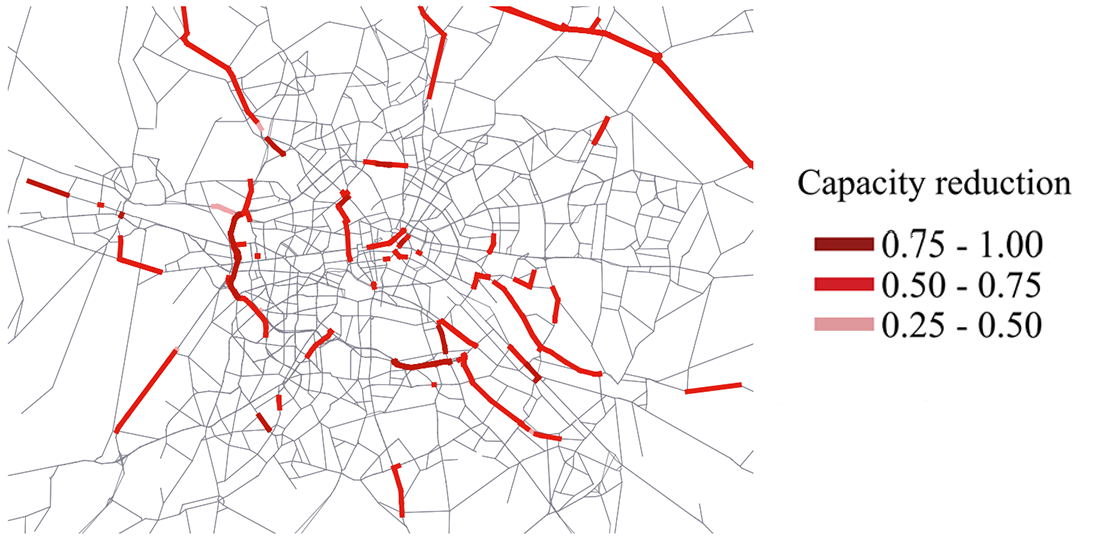
\includegraphics{figures/berlin_capacity.png}

}

\caption{\label{fig-berlin_cap}Traffic incidents mapped on the Berlin
network.}

\end{figure}

Kaddoura \& Nagel (2018) found that long-term traffic incidents increase
traffic congestion and the average car travel time by 313 sec (+18\%)
per trip. Short-term traffic incidents increase the average travel time
per car trip by another 136 sec (+8\%). Additionally, they found that
for 44\% of all car trips, the agent's transport route contained at
least one road segment for which the capacity or speed limit was reduced
because of an incident. Their study concluded that networks in which
transport users had high levels of knowledge about the incidents and
resulting traffic congestion still experienced an increase in travel
time caused by long and short-term incidents. Finally, Kaddoura and
Nagel asserted that ``accounting for traffic incidents makes the model
more realistic, allowing for an improved policy investigation''
(Kaddoura \& Nagel, 2018, p. 885). The modeling performed by Kaddoura
and Nagel is just one example of research on MATSim's capacity for
incident-based simulations

A MATSim incidents model developed by Li \& Ferguson (2020) included
various rescheduling options, such as departure time, mode choice, and
trip cancellation. Their simulation found that if travelers received
notice of an incident, they would either depart early from their place
of origin or switch to public transport (Li \& Ferguson, 2020). The
process proposed by Li and Ferguson is beneficial because it allows
agents to reassess their mode choice or route assignment based on the
notice of a reported incident. Li and Ferguson show that users care
about total travel time and travel time variability (risk tolerance to a
certain degree). Receiving notifications about incidents by agents
impacted both travel time and mode choice. They concluded that ``the
provision of real-time traffic information is a useful approach to
mitigating the side-effects of incidents through helping transport users
efficiently adapt their day plans'' (Li \& Ferguson, 2020, p. 96).
Additionally, they found that ``most of the travelers notified of being
affected by incidents are simulated to depart early or switch to public
transport, which effectively reduces the average travel time delay
caused by disruptions'' (Li \& Ferguson, 2020, p. 96). Their findings
validate the conclusions of Sisiopiku et al. (2007) that making incident
information available to agents leads to decreases in travel time and
congestion.

This subsection highlight the capabilities of DTA models to simulate the
complexities of traffic incidents, congestion, and travel times. It
highlights how incorporating incident management responses into the
models would enhance their ability to simulate realistic traffic
conditions and support policy analysis. Given its capacity to model
large-scale networks, integrate real-world data, and replicate realistic
driver behavior, MATSim is deemed particularly suitable for this
project. It will be employed to assess the effectiveness of IMT in Utah.

\hypertarget{sec-lit_summary}{%
\section{Summary}\label{sec-lit_summary}}

\protect\hyperlink{sec-literature}{Literature Review} provides an
overview of the extensive research on the effectiveness of IMT in
reducing RCT and ECU during incident responses. It has also highlighted
studies focused on optimizing the size and distribution of IMT. However,
these studies do not include the broader implications of incidents and
IMT responses on large-scale networks and their agents. On the other
hand, while DTA modeling studies have effectively explored the impact of
incidents on network dynamics and driver behavior, they largely have not
examined the influence of IMT. This creates a research gap in
understanding the effectiveness of IMT and the impact of incidents on
congested networks. Bridging this gap is crucial, as it enables
researchers to better grasp how alterations in incident occurrence or
IMT availability might influence overall traffic conditions. In our
research, we aim to merge these two areas of study, attempting to model
incident response within a simulation framework, thereby broadening the
scope for evaluating IMT deployment strategies and their effectiveness.

\bookmarksetup{startatroot}

\hypertarget{sec-methods}{%
\chapter{Methodology}\label{sec-methods}}

As highlighted in the \protect\hyperlink{sec-literature}{Literature
Review}, there is substantial evidence indicating that IMT can
effectively reduce RCT and ECU following traffic incidents.
Additionally, the effectiveness of DTA models in analyzing the impact of
such incidents has been well-documented. However, there is a lack of
comprehensive research evaluating IMT impact on entire traffic networks
and their associated agents. To address this gap, it is necessary that
we develop a model capable of simulating both traffic incidents and the
ensuing IMT interventions, with the objective of gauging the efficiency
of IMT deployments. Due to its proficiency in regional-scale incident
simulation and its authentic portrayal of driver behavior, MATSim has
been identified as the most suitable model for this research. This
section describes the methodology, expounding on the model's
capabilities, the requisite data inputs, and the benchmarks established
for determining IMT effectiveness.

Our methodology is structured around three main components: the
functionality of the MATSim model, the setup of IMT vehicles and
incidents, and the scenarios for comparative analysis. In
\protect\hyperlink{sec-MATSim_mod}{Model Design} we describe the
structure of the model and the functions it uses to represent incidents
and IMT response. In \protect\hyperlink{sec-model_imp}{Model
Implementaiton} we outline the data structure of the model by first
describing \protect\hyperlink{sec-IMT_setup}{IMT Setup}, then
\protect\hyperlink{sec-inc_data}{Incident Data and Sampling} and
conclude by describing the \protect\hyperlink{sec-scenarios}{Scenarios}
used for evaluating the impact of incidents and IMT.

\hypertarget{sec-MATSim_mod}{%
\section{Model Design}\label{sec-MATSim_mod}}

MATSim is an open-source framework used for conducting extensive,
agent-based transportation simulations on a large scale. Operating as a
dynamic traffic simulation, it is often used in demand modeling and
agent-based mobility analysis (Dobler \& Nagel, 2016). Thanks to its
open-source architecture, MATSim enables the seamless integration of a
diverse array of modules and packages into its models. Users across the
platform can create, import, and modify these components, fostering a
collaborative and innovative environment.

For the purposes of our research, we developed the ImtModule, a
specialized MATSim extension designed to process incidents and IMT
responses within the simulation. This module leverages existing research
on incident simulation, Demand Rapid Transit (DRT), event handling, and
vehicle dispatch algorithms, building upon these foundations to enhance
the functionality of our model.

In this section, we describe some of the specific tools within MATSim
that we used and adapted to construct a comprehensive and functional
model. These tools include \protect\hyperlink{sec-MATSim_score}{Scoring
and Replanning}, \protect\hyperlink{sec-NCE}{Network Change Events}, and
\protect\hyperlink{sec-imt_response}{IMT Assignment and Response}.
Together, they contribute to the realism and precision of our traffic
simulations, particularly in the context of responding to roadway
incidents, ensuring that our model provides accurate and reliable
results.

\hypertarget{sec-MATSim_Score}{%
\subsection{Scoring and Replanning}\label{sec-MATSim_Score}}

In MATSim, each individual within the simulation is called an agent.
These agents follow daily schedules, partaking in various activities and
modes of travel. Their actions are evaluated using a point system, which
takes into account the specifics of their travel, as highlighted by
Nagel et al. (2016). Timely arrivals at destinations are rewarded with
positive points, whereas delays result in deductions. Furthermore,
different transportation modes are assigned utility scores, which play a
crucial role in shaping the agents' travel preferences and decisions.

Each agent possesses a memory that stores plans from a certain number of
iterations, as well as replanning strategies that dictate how agents can
adjust their plans from iteration to iteration Horni \& Nagel (2016).
The size of an agent's memory is typically dependent on the size of the
model being run. In the case of our large-scale Utah model, we opted to
limit the agents' plan memory to just five iterations. The replanning
strategies used include selecting the plan with the highest score 80\%
of the time, opting to reroute 10\% of the time, and adjusting activity
timings for the remaining 10\%. Our selection for the remaining scoring
and replanning parameters drew from the incident research conducted by
Kaddoura \& Nagel (2018).

Each agent possesses a memory that stores plans from a certain number of
iterations, as well as replanning strategies that dictate how agents can
adjust their plans from iteration to iteration Horni \& Nagel (2016).
The size of an agent's memory is typically dependent on the size of the
model being run. In the case of our large-scale Utah model, we opted to
limit the agents' plan memory to just five iterations. The replanning
strategies used include selecting the plan with the highest score 80\%
of the time, opting to reroute 10\% of the time, and adjusting activity
timings for the remaining 10\%. The remaining scoring and replanning
parameters were primarily selected based on insights from the incident
research conducted Kaddoura \& Nagel (2018) and the parameters used in
their model.

As detailed in \protect\hyperlink{sec-model_imp}{Model Implementaiton},
the plans file used to generate simulations in MATSim was considerably
massive, encapsulating travel data for over 2 million agents. Our
objective, utilizing the complete plans file, was to guide the simulated
agents toward an equilibrium in travel behavior. To achieve this, we
employed the following methodology: 1. We processed both the network and
plans files over the course of 350 simulated iterations with incidents
or IMT included. 2. Using the output from this preliminary scenario, we
established a `hot start' for the subsequent scenarios incorporating
incidents and IMT responses. At this stage, a significant portion of
agents had already identified efficient travel routes to their
destinations. This preliminary phase of running the plans file was
intended to expedite the convergence towards a balanced state in travel
behavior for scenarios that included incidents and IMT responses. 3. To
achieve equilibrium in travel behavior, we conducted an additional 100
iterations in the simulations that accounted for incidents and IMT
responses, ensuring a more comprehensive stabilization across the
majority of scenarios.

\hypertarget{sec-NCE}{%
\subsection{Network Change Events}\label{sec-NCE}}

Within a MATSim network, each link is characterized by specific
attributes such as type, length, number of lanes, free-flow speed, and
capacity. To effectively simulate unexpected events and their subsequent
impacts on traffic flow, it is essential to dynamically adjust these
attributes. This capability, termed a Time-Dependent Network, is
explained in the MATSim textbook (Rieser, 2016) and is vital for
ensuring the realism and accuracy of our simulation.

Network Change Events (NCE) serve as the mechanism within MATSim for
modifying network attributes at precise moments during a simulation.
Detailed in Section 6.1 of the MATSim textbook (Rieser, 2016), the
implementation of NCE requires specific adjustments to the MATSim
configuration file to facilitate a time-variant network. These events
can modify a link's free-flow speed, number of lanes, or capacity. To
initiate a network change event, the system requires specific
information including the time of the event \texttt{startTime}, the
affected link(s) \texttt{link\ refID}, the type of change
\texttt{free-flow\ speed}, \texttt{lanes}, or \texttt{capacity}, and the
value of the change. NCE are the tools used in this study to demonstrate
the impact of both incidents and IMT arrivals.

\hypertarget{sec-imt_response}{%
\subsection{IMT Assignment and Response}\label{sec-imt_response}}

Within MATSim, the dispatch of one or more IMT is triggered by the
occurrence of an incident. The optimal IMT for the situation is
determined using a least-cost path dispatch algorithm, which bases its
calculations on vehicle paths while considering factors such as
congestion and link speed. The success of these methods heavily relies
on the IMT units' capability to navigate through traffic. In cases where
all IMT are occupied at the time of an incident, the algorithm waits
until a vehicle becomes available, and subsequently dispatches it to the
incident site.

Upon an IMT's arrival at an incident, a NCE is activated via an event
handler, a MATSim tool that functions to log simulation events in
real-time. While incidents reduce a link's capacity, the IMT's arrival
triggers a NCE that restores 25\% of the capacity gap on the affected
link. The capacity gap is defined as the difference between the link's
full capacity and its reduced capacity during an incident. For incidents
requiring the response of multiple IMT, each arriving unit restores an
additional 25\% of the existing capacity gap.

Figure~\ref{fig-imt_capacity_restore} demonstrates the potential impact
of an incident lacking IMT intervention, compared with scenarios that
include the response of one or two IMT. This illustration highlights the
critical role of IMT, showcasing their ability to mitigate incident
impacts on network traffic flow.

\begin{figure}

{\centering \includegraphics{03_methods_files/figure-pdf/fig-imt_capacity_restore-1.pdf}

}

\caption{\label{fig-imt_capacity_restore}IMT capacity restoration upon
arrival example.}

\end{figure}

\hypertarget{sec-model_imp}{%
\section{Model Implementaiton}\label{sec-model_imp}}

To run the MATSim model with the ImtModule extension, a number of input
resources are necessary. For the model to function properly, the
following are needed:

\begin{itemize}
\tightlist
\item
  A plans file detailing the agents to be modeled, as well as their
  origins and destinations.
\item
  A network file with interconnected links, enabling travel for the
  agents specified in the plans file.
\item
  A configuration file outlining the scoring metrics of the simulation
  and establishing parameters pertaining to agent and IMT travel
  patterns.
\item
  An IMT file outlining the IMT starting locations and hours of
  operation.
\item
  An incidents file containing the necessary data to randomly effect NCE
  throughout the simulation.
\end{itemize}

The network and plans files used in this research were developed and
calibrated by Lant (2021) and Day (2022) as part of their research
projects studying accessibility and ride-hailing throughout the Wasatch
Front. The configuration file used in the model was adapted from the
Kaddoura \& Nagel (2018) file, which was used for their MATSim incident
analysis study. It was slightly modified to accommodate the IMT
development, but the parameters they set were largely left unaltered.
The IMT file was produced using data provided by UDOT and UHP, as
outline in \protect\hyperlink{sec-MATSim_mod}{IMT Setup}. The incident
data was compiled by Hyer (2023) in his research of IMT performance
measures and is explained in \protect\hyperlink{sec-inc_data}{Incident
Data and Sampling}.

\hypertarget{sec-IMT_setup}{%
\subsection{IMT Setup}\label{sec-IMT_setup}}

UDOT currently operates a fleet of 20 IMT, distributed across three
zones corresponding to Davis, Salt Lake, and Utah counties within the
Wasatch Front. Figure~\ref{fig-IMT_Map} provides a visual representation
of the county boundaries and the initial locations of both existing and
newly proposed IMT vehicles used in the simulation.

\begin{figure}

{\centering 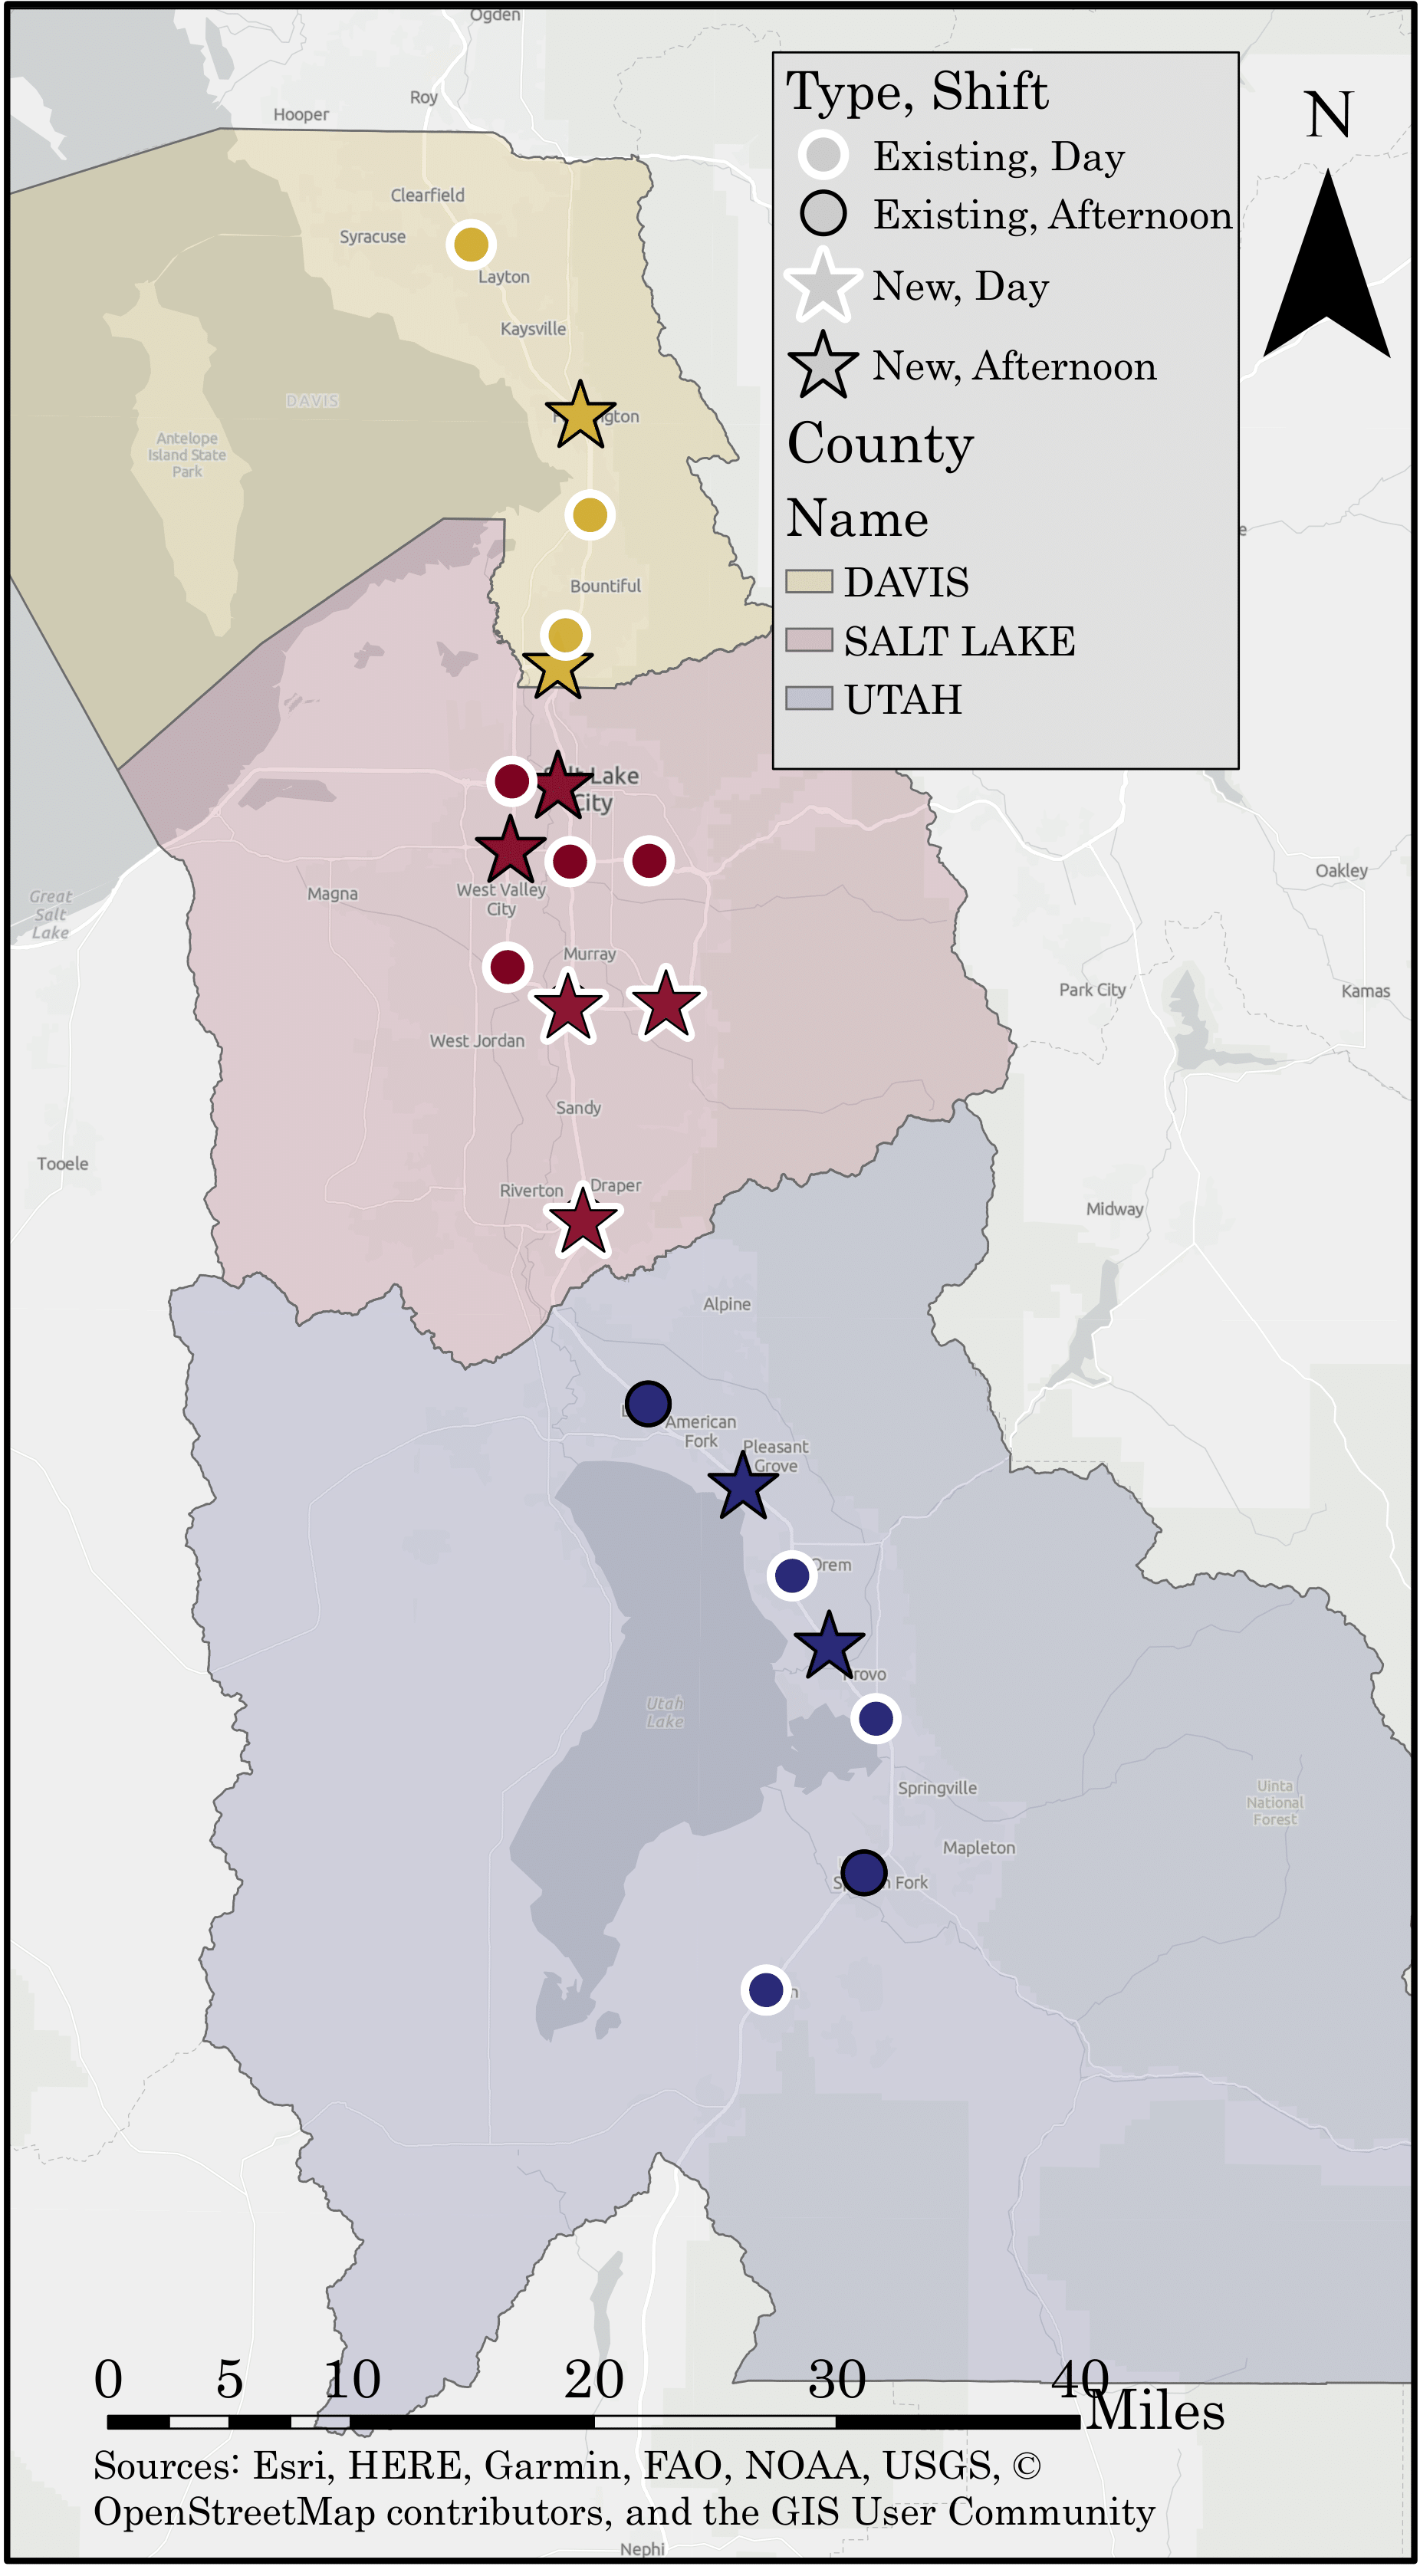
\includegraphics{figures/imt_gray_map.png}

}

\caption{\label{fig-IMT_Map}IMT starting locations example map.}

\end{figure}

In Figure~\ref{fig-IMT_Map}, circles indicate the locations of existing
IMT vehicles, while stars denote the proposed additions. These initial
positions are carefully selected to maintain a uniform distribution of
IMT vehicles across each county. Typically, IMT vehicles do not cross
county borders during operations since dispatch services are organized
at the county level. However, our MATSim network does not enforce such
restrictions, permitting vehicles to traverse county lines based on the
proximity of incidents. The specific starting points are noted in the
IMT file as starting links, streamlining their integration into MATSim.
While Figure~\ref{fig-IMT_Map} showcases the IMT distribution during the
evening shift, it is crucial to highlight that IMT distribution remains
largely unaltered throughout the morning and afternoon shifts. The
initial setup of IMT, although it does not replicate the real-world
scenario of drivers beginning their shifts from home, provides a viable
solution for our simulations. Considering the significant number of IMT
operations along major highways such as I-15, I-80, and I-215, and the
daily variations in real-world starting locations, this strategic
placement along key routes is justified. In the 30 IMT scenario, all
vehicles from the 20 IMT scenarios are retained and augmented with an
additional 10 IMT, ensuring comprehensive coverage across all three
counties.

Our research primarily concentrates on evaluating the potential impacts
of expanding the IMT fleet, rather than examining the effects of their
starting positions. We hypothesize that increasing the number of IMT,
assuming uniform distribution, will enhance their overall effectiveness.

\hypertarget{sec-inc_data}{%
\subsection{Incident Data and Sampling}\label{sec-inc_data}}

Hyer (2023) undertook concurrent IMT research and compiled a
comprehensive dataset of incidents requiring IMT intervention, drawing
on data from the UHP. He carefully ensured the completeness of each
incident record in the dataset, capturing crucial details such as the
incident start and end times, RCT, location, and extent of capacity
reduction.

Analyzing data from 2018 and 2022, Hyer (2023) successfully identified
411 unique incidents with varying degrees of severity, ranging from
property damage to fatal incidents. We utilized this carefully curated
dataset to selectively include specific incidents in the MATSim model.
It is important to acknowledge that these 411 incidents only constitute
a portion of all incidents reported by UHP during this time frame. A
significant number of additional incidents were not considered in the
analysis due to the absence of vital metrics necessary for a
comprehensive evaluation (e.g., start time, RCT, etc.). Nevertheless,
the integration of the 411 analyzed incidents with the additional
incomplete records provides insights, aiding in quantifying the total
number of incidents within a specific time period. These combined
incident records were used in modeling daily incident frequencies.

To generate ten distinct values representing daily incident frequencies,
we employed a randomized sampling technique. These values were
collectively termed Current Incident Frequencies as they were derived
from the original distribution of daily incidents. Furthermore, we
formulated a second set of ten daily incident values, named Increased
Incident Frequencies. These values were extracted from the upper portion
of the 2022 incident data and were specifically designed to assess the
resilience and efficacy of the IMT system under scenarios of markedly
increased daily incidents. The visual depiction of the original
distribution of daily incidents, alongside the distributions for both
the Current and Increased Incident Frequencies, is illustrated in
Figure~\ref{fig-incident_sampling_plot}.

\begin{figure}

{\centering \includegraphics{03_methods_files/figure-pdf/fig-incident_sampling_plot-1.pdf}

}

\caption{\label{fig-incident_sampling_plot}Sampling distributions for
incident frequencies.}

\end{figure}

In total, twenty values were selected, evenly split with ten allocated
to the Current Incident Frequency category, and the remaining ten to the
Increased Incident Frequency category. Each value was subsequently
paired with a unique three-digit seed number, utilized internally within
MATSim to ensure a randomized selection of incidents for each simulation
scenario. Following this, we employed the MATSim
\protect\hyperlink{sec-NCE}{Network Change Events} to integrate the
incidents into the simulation.

\hypertarget{sec-scenarios}{%
\subsection{Scenarios}\label{sec-scenarios}}

In \protect\hyperlink{sec-inc_data}{Incident Data and Sampling} and
Figure~\ref{fig-incident_sampling_plot}, we observe the establishment
and categorization of twenty distinct incident seeds into either Current
or Increased Incident frequencies. Each seed gave rise to three separate
simulation groups. The first group, No IMT, exclusively features
simulations where incidents occur without any IMT intervention. The
second group includes incidents and the deployment of 20 IMT, while the
third group features incidents managed by 30 IMT. To facilitate
efficient organization and comparative analysis, each scenario was
assigned a unique identifier, such as ``1-10-257.'' Within this coding
system, the first digit specifies the simulation group (No IMT, 20 IMT,
or 30 IMT), the second denotes the number of incidents included in the
simulation, and the third digit corresponds to the seed value utilized
for random incident selection.

In total, six scenario groups were established, as follows:

\begin{itemize}
\tightlist
\item
  No IMT, current incident frequency
\item
  No IMT, increased incident frequency
\item
  20 IMT, current incident frequency
\item
  20 IMT, increased incident frequency
\item
  30 IMT, current incident frequency
\item
  30 IMT, increased incident frequency
\end{itemize}

It is important to note, as described in
\protect\hyperlink{sec-IMT_setup}{IMT Setup}, that not all IMT vehicles
are operational simultaneously. Due to scheduling constraints, the
actual number of IMT on the road at any given time is typically half of
the total fleet size.

The study utilizes the MATSim model for conducting simulations across
all three groups: No IMT, 20 IMT, and 30 IMT. Each simulation underwent
an internal comparison, as well as comparison against a Baseline
scenario devoid of incidents or IMT intervention. This comprehensive
analysis affords a holistic approach in assessing IMT effects on traffic
dynamics and their operational efficiency.

The primary metric for traffic impact analysis in this study is the
total vehicle hours of delay (VHD), dissected through three
investigative tiers: Network Links, Motorway Links, and Impacted Links.
Network Links offer a macroscopic view of the network-wide delay,
Motorway Links focused on major highways and freeways, and Impacted
Links provide a microscopic view of the delays at incident sites and
their immediate upstream links. This tiered approach ensures a thorough
analysis, capturing the overarching impact on traffic flow while also
honing in on critical areas affected by incidents.

In addition to VHD, the study investigates the performance and
operational efficiency of IMT. Metrics such as the average travel times,
travel distances, and incident response times of IMT are compared across
the 20 IMT and 30 IMT groups. This, in turn, informs strategic decisions
regarding resource allocation and deployment, ensuring that IMT vehicles
are optimally utilized to mitigate traffic delays and enhance roadway
safety.

\bookmarksetup{startatroot}

\hypertarget{sec-results}{%
\chapter{Results}\label{sec-results}}

This section details the outcomes of the Utah IMT Optimization project,
employing the MATSim model to execute a series of simulations across a
range of scenario groups. Specifically, the groups---No IMT, 20 IMT, and
30 IMT---were compared with a Baseline scenario, facilitating an
evaluation of the repercussions of traffic incidents and the
effectiveness of IMT in alleviating traffic disruptions.

The following sections analyze the results derived from the simulated
scenarios. This analysis uses comparative metrics such as vehicle hours
of delay (VHD), the consequences of traffic incidents, and the dynamics
of the IMT responses in relation to the incidents they manage.

\hypertarget{vehicle-hours-of-delay}{%
\section{Vehicle Hours of Delay}\label{vehicle-hours-of-delay}}

The studies referenced in the \protect\hyperlink{sec-lit_imt_opt}{IMT
Optimization} section of the
\protect\hyperlink{sec-literature}{Literature Review} demonstrate the
efficacy of IMT in reducing RCT and ECU on roadway segments affected by
incidents. Similarly, the results from this transportation model
highlight the impact of IMT at reducing delay, particularly when
focusing on the segments of roadways where incidents occurred; see
\protect\hyperlink{sec-impacted}{Impacted Links}. In contrast to the
cited studies, our model also explored the broader implications of
incidents and their corresponding IMT responses on the simulated
network. In a majority of scenarios, these results also indicated a
positive correlation between IMT response and a decrease in VHD.

\hypertarget{network-hours-of-delay}{%
\subsection{Network Hours of Delay}\label{network-hours-of-delay}}

In the comparison of network VHD across simulations, the scenarios were
grouped by IMT response and incident frequency. Each group encompassed
ten simulated scenarios, which involved different selections of
incidents, with the exception of the Baseline scenario, which stands
alone. Table~\ref{tbl-network_delays_table} presents the average VHD for
each group, based on the delays recorded in the final iteration of each
simulation. These average VHD values are subsequently compared against
the Baseline scenario to calculate the percentage change in VHD.

\hypertarget{tbl-network_delays_table}{}
\begin{table}
\caption{\label{tbl-network_delays_table}Average Delay on Network }\tabularnewline

\centering
\begin{tabular}[t]{llrr}
\toprule
\textbf{Group} & \textbf{Incident Frequency} & \textbf{Average VHD} & \textbf{Change (\%)}\\
\midrule
\cellcolor{gray!6}{Baseline} & \cellcolor{gray!6}{-} & \cellcolor{gray!6}{74568} & \cellcolor{gray!6}{0.0}\\
No IMT & Current & 103159 & 38.3\\
\cellcolor{gray!6}{No IMT} & \cellcolor{gray!6}{Increased} & \cellcolor{gray!6}{104178} & \cellcolor{gray!6}{39.7}\\
20 IMT & Current & 96697 & 29.7\\
\cellcolor{gray!6}{20 IMT} & \cellcolor{gray!6}{Increased} & \cellcolor{gray!6}{95678} & \cellcolor{gray!6}{28.3}\\
\addlinespace
30 IMT & Current & 93769 & 25.7\\
\cellcolor{gray!6}{30 IMT} & \cellcolor{gray!6}{Increased} & \cellcolor{gray!6}{93560} & \cellcolor{gray!6}{25.5}\\
\bottomrule
\end{tabular}
\end{table}

Upon comparing the results across different groups, it was observed that
scenarios with 30 IMT experienced the lowest average VHD. They were
closely followed by the 20 IMT group, and, as expected, the scenarios
that involved incidents only registered the highest average VHD values.
It is also noted that introducing incidents to the baseline scenario
resulted in an average VHD increase of 39\%. However, this increase
dropped to an average of 29\% when 20 IMT were available, and further
reduced to 25.6\% with the availability of 30 IMT.

Additional analysis of the data revealed that, compared to the No IMT
group, the 20 IMT group decreased the average VHD by 7.2\%, while the 30
IMT group reduced the average delay by 9.6\%. Lastly, when the 30 IMT
and 20 IMT groups were compared against each other, the former exhibited
an average of 2.6\% less VHD than the latter.

While the relationship between the IMT group and VHD appeared
straightforward, the correlation between Incident Frequency and VHD was
not as clear-cut. In the No IMT group, scenarios with increased incident
frequency showed only a one percent increase in VHD compared to those
with the current frequency. Intriguingly, for both the 20 IMT and 30 IMT
groups, an increase in incident frequency actually led to slight
decreases in average VHD. The cause of this decrease is unclear, but
potential explanations will be discussed in
\protect\hyperlink{sec-limitations}{Limiations}.

Given that Table~\ref{tbl-network_delays_table} reveals average delay
values aggregated across multiple scenarios within each group, a
graphical representation can enhance clarity regarding the inherent
variance within these data clusters.
Figure~\ref{fig-network_violin_plot} illustrates this data through
violin plots.

\begin{figure}

{\centering \includegraphics{04_results_files/figure-pdf/fig-network_violin_plot-1.pdf}

}

\caption{\label{fig-network_violin_plot}Average network delay violins.}

\end{figure}

In Figure~\ref{fig-network_violin_plot}, each violin plot represents the
density distribution of delay values, with wider sections indicating
areas where numerous simulations converged around specific delay values.
Conversely, narrower sections suggest fewer simulations clustering
around those particular delay values. A dashed horizontal line is
superimposed to facilitate comparison of each group with the results
from the Baseline scenario. Additionally, diamond markers within each
plot denote the mean delay across all simulations in the respective
scenario group.

Upon examining these violin plots, several observations can be made. In
the No IMT group, the distribution of delay values has a relatively
narrow spread at the lower end, widening around the 100,000 mark, with
the mean delay slightly skewed toward 104,000. This skew is influenced
by some values that approach 120,000 hours of delay. In contrast, the 20
IMT group exhibits significant variability, as reflected by its
consistent width across the range of values. The scenarios within the 30
IMT group show marginally reduced variability compared to the 20 IMT
group and feature distinct concentrations around 90,000 VHD and 100,000
VHD.

While the preceding section discussed delays across the entire network,
it is important to note that all simulated incidents were located on
motorway links, predominantly along the major interstates of Utah's
Wasatch Front. This encompasses key routes such as I-15, I-80, and
I-215, as well as other significant freeways and highways. The
subsequent section will provide a detailed analysis of the simulation
outcomes specifically related to these motorway links.

\hypertarget{motorway-link-hours-of-delay}{%
\subsection{Motorway Link Hours of
Delay}\label{motorway-link-hours-of-delay}}

The network used in our model is derived from an OpenStreetMap, which
Lant (2021) and Day (2022) also utilized for their research projects.
Within this network, the term `motorway' denotes a specific type of
link, also known as a freeway or expressway in different contexts. To
ensure consistency throughout this document, we primarily refer to these
road segments as `motorway' or `motorway links'. It is important to
note, however, that in the simulation, incidents can occur on both
interstates and major highways along the Wasatch Front.

To compare average simulation performances,
Table~\ref{tbl-motorway_delays_table} breaks down the average Motorway
VHD for each group, categorized by IMT response and incident frequency.

\hypertarget{tbl-motorway_delays_table}{}
\begin{table}
\caption{\label{tbl-motorway_delays_table}Average VHD of Motorway Links }\tabularnewline

\centering
\begin{tabular}[t]{llrr}
\toprule
\textbf{Group} & \textbf{Incident Frequency} & \textbf{Average VHD} & \textbf{Change (\%)}\\
\midrule
\cellcolor{gray!6}{Baseline} & \cellcolor{gray!6}{-} & \cellcolor{gray!6}{15335} & \cellcolor{gray!6}{0.0}\\
No IMT & Current & 24242 & 58.1\\
\cellcolor{gray!6}{No IMT} & \cellcolor{gray!6}{Increased} & \cellcolor{gray!6}{22321} & \cellcolor{gray!6}{45.6}\\
20 IMT & Current & 18924 & 23.4\\
\cellcolor{gray!6}{20 IMT} & \cellcolor{gray!6}{Increased} & \cellcolor{gray!6}{19176} & \cellcolor{gray!6}{25.0}\\
\addlinespace
30 IMT & Current & 17569 & 14.6\\
\cellcolor{gray!6}{30 IMT} & \cellcolor{gray!6}{Increased} & \cellcolor{gray!6}{18327} & \cellcolor{gray!6}{19.5}\\
\bottomrule
\end{tabular}
\end{table}

Table~\ref{tbl-motorway_delays_table} reveals that, in comparison to the
Baseline scenario, the average VHD on motorway links increased by
approximately 7,000-9,000 hours, or 45.6-58.1\%, when incidents were
introduced. The 20 IMT group, on average, exhibited a 24.2\% increase in
VHD from the Baseline, whereas the 30 IMT group experienced an average
VHD increase of 17\%.

At the motorway link level, the differences between the No IMT group and
the IMT groups becomes more pronounced they were for delays across the
entire network. Specifically, the 20 IMT group demonstrated an average
18.2\% decrease in VHD compared to the No IMT group, while the 30 IMT
group showed an average 22.9\% decrease in VHD.

Interestingly, the difficulty in correlating VHD with incident frequency
observed in Table~\ref{tbl-network_delays_table} manifests differently
in Table~\ref{tbl-motorway_delays_table}. The latter indicates that,
within the IMT groups, an increase in incident frequency corresponds
with an increase in VHD. Specifically, the 20 IMT group experiences an
average VHD increase of 1.3\% when transitioning from current to
increased incident frequencies, while the 30 IMT group sees a 4.3\%
uptick under the same conditions. In contrast, and quite unexpectedly,
the No IMT group shows a 7.9\% reduction in VHD when comparing scenarios
of current and increased incident frequencies. This finding is
particularly perplexing given that Table~\ref{tbl-network_delays_table}
suggests an overall increase in VHD across the entire network for the No
IMT group when incident frequency increases.

A potential explanation for these unexpected VHD outcomes on motorway
links could be that, as part of their scoring and replanning process,
some MATSim agents opted for travel on non-motorway links to reach their
destinations. This would essentially redistribute the delay from
motorway links to other parts of the network.

For a better understanding of the variances within the scenario groups,
Figure~\ref{fig-motorway_violin_plot} may provide additional insights.

\begin{figure}

{\centering \includegraphics{04_results_files/figure-pdf/fig-motorway_violin_plot-1.pdf}

}

\caption{\label{fig-motorway_violin_plot}Average motorway delay
violins.}

\end{figure}

In Figure~\ref{fig-motorway_violin_plot}, we observe distinct patterns
in the distribution of delays for different scenario groupings. Key
observations include:

\begin{itemize}
\tightlist
\item
  A wide span across the plots for both groupings of No IMT, indicating
  a significant variance in delays across those simulations.
\item
  A concentration of delays around the Baseline value of 15,000 VHD for
  both the 20 IMT and 30 IMT scenarios, as shown by the width of the
  plots at this point.
\item
  A narrowing of the IMT group plots as they transition to higher delay
  values, suggesting fewer instances of extreme delays.
\item
  The upper tails of the 20 IMT plots extend beyond those of the 30 IMT
  plots, suggesting that the 30 IMT fleet may be more effective at
  mitigating delays in outlier scenarios compared to the 20 IMT fleet.
\end{itemize}

The final section of our VHD analysis delves into the delays experienced
on incident links and their immediate upstream counterparts. This level
of analysis aligns with the methodologies employed in the studies by
Schultz et al. (2019) and Skabardonis et al. (1998), as it focuses on
the most direct repercussions of incidents and IMT. Unlike their focus
on the impacts of IMT on RCT and ECU, our investigation centers on VHD.
As detailed in \protect\hyperlink{sec-imt_response}{IMT Assignment and
Response}, the IMT in our simulation did not curtail the duration of
incidents (RCT); instead, they enhanced roadway capacity. Nonetheless,
given that ECU is intrinsically related to delay,
\protect\hyperlink{sec-impacted}{Impacted Links} offers an evaluation of
IMT performance similar to the analyses conducted by Schultz et al.
(2019) and Skabardonis et al. (1998).

\hypertarget{sec-impacted}{%
\subsection{Impacted Links}\label{sec-impacted}}

Impacted Links examines VHD on incident links and their immediate
upstream counterparts. Given the variation in link lengths across the
motorway, in some cases, analyzing just two additional links may not
fully capture the delays caused by a specific incident. Nevertheless,
Table~\ref{tbl-impacted_links} provides insights into how delays on
impacted links vary based on incidents and IMT deployment. For
additional context about Table~\ref{tbl-impacted_links}: `Total VHD'
represents the delay on impacted links both during the incidents and for
one hour after clearance, aiming to capture any residual delay shock
waves that an incident might cause.

\hypertarget{tbl-impacted_links}{}
\begin{table}
\caption{\label{tbl-impacted_links}Impacted Links Delay }\tabularnewline

\centering
\begin{tabular}[t]{llrr}
\toprule
\textbf{Group} & \textbf{Incident Frequency} & \textbf{Total VHD} & \textbf{Avg. Delay Per Inc. [hrs.]}\\
\midrule
\cellcolor{gray!6}{Baseline} & \cellcolor{gray!6}{Current} & \cellcolor{gray!6}{326} & \cellcolor{gray!6}{3.6}\\
No IMT & Current & 3808 & 42.3\\
\cellcolor{gray!6}{20 IMT} & \cellcolor{gray!6}{Current} & \cellcolor{gray!6}{723} & \cellcolor{gray!6}{8.0}\\
30 IMT & Current & 366 & 4.1\\
\cellcolor{gray!6}{Baseline} & \cellcolor{gray!6}{Increased} & \cellcolor{gray!6}{540} & \cellcolor{gray!6}{2.8}\\
\addlinespace
No IMT & Increased & 3154 & 16.3\\
\cellcolor{gray!6}{20 IMT} & \cellcolor{gray!6}{Increased} & \cellcolor{gray!6}{1645} & \cellcolor{gray!6}{8.5}\\
30 IMT & Increased & 1115 & 5.8\\
\bottomrule
\multicolumn{4}{l}{\textsuperscript{a} Note: Current contains 90 incidents, Increased contains 193}\\
\end{tabular}
\end{table}

Table~\ref{tbl-impacted_links} presents a division of the Baseline
scenario into two segments, for a more accurate comparison with the
other three scenarios. Despite the absence of incidents in the Baseline
scenario, its delay values are derived from the same links included in
the other scenarios.

The data in Table~\ref{tbl-impacted_links} indicate that the 30 IMT
group delay patterns align most closely with the baseline. They are
followed by the 20 IMT group, and subsequently, the No IMT group. It is
important to note that directly comparing the Total VHD of the Current
and Increased incident groups may not be appropriate due to variations
in sample sizes, as underscored by Table~\ref{tbl-impacted_links}. A
more apt comparison might be to evaluate the average delay experienced
per incident. Using this parameter, we observe an increase in the
average VHD for both the 20 and 30 IMT groups, correlating with an
uptick in the number of incidents. However, the scenarios involving No
IMT yield a different outcome: both Total VHD and the average delay per
incident exhibit a decrease when the incident frequency increased. A
more close examination of the data draws attention to a particular
scenario, Seed 141, which contributed an exceptionally large delay to
the incident links in the Current Incident category. This anomaly could
potentially explain the seemingly unexpected findings observed in the No
IMT, Current Incident frequency scenarios.

For a more detailed analysis, the scatter plot in
Figure~\ref{fig-impacted_links_plot} categorizes the data based on seed
type. On the y-axis, the labels represent a combination of incident
numbers and seed values, with the format ``number\_seed'' (e.g.,
``12\_141'' denotes a scenario involving 12 incidents associated with
seed value 141).

\begin{figure}

{\centering \includegraphics{04_results_files/figure-pdf/fig-impacted_links_plot-1.pdf}

}

\caption{\label{fig-impacted_links_plot}Delay on impacted links sorted
by seed.}

\end{figure}

Figure~\ref{fig-impacted_links_plot} offers a detailed view of the VHD
on impacted links across the simulated scenarios. At a glance, the
Baseline and 30 IMT scenarios, represented by blue and orange dots, seem
to predominantly cluster to the left of the pink dots, which depict the
No IMT scenarios. However, a more thorough analysis reveals that in
specific instances, the 20 IMT, 30 IMT, or even both scenarios may
underperform compared to the No IMT scenarios. This seemingly unexpected
observation suggests that there may be additional factors, aside from
link capacity, affecting the delay.

It is important to acknowledge the inherent dynamic nature of the MATSim
iterative process, where the ways in which agents re-plan their journeys
can sometimes have as significant, or potentially even greater, impact
on delays than changes in link capacity due to incidents or IMT.
Importantly, in scenarios with the highest delays, the introduction of
IMT seems to considerably reduce delay on the affected links.

Note that the x-axis has been limited to a maximum of 400+ VHD. This
limit enhances the visibility of the majority of data points. Without
this adjustment, the outlier point from the No IMT scenario with seed
141, which reported over 1,000 hours of delay, would have necessitated a
much wider scale, potentially obscuring the trends and patterns in the
rest of the data.

\hypertarget{imt-vehicle-analysis}{%
\section{IMT Vehicle Analysis}\label{imt-vehicle-analysis}}

Equally critical to understanding IMT performance is assessing the
efficiency of each IMT in reaching their intended destinations. This
results segment delves into IMT travel behavior, capturing metrics such
as average travel times and distances, along with their average incident
response times. The analysis encompasses both 20 IMT and 30 IMT
scenarios.

\hypertarget{imt-travel-time}{%
\subsection{IMT Travel Time}\label{imt-travel-time}}

Travel times for IMT can be extracted from the event files, which are
produced as a standard MATSim output. These files provide insights into
the distance and time traveled by each IMT. Utilizing this IMT travel
data, plots were generated to illustrate the average travel times and
distances for each dispatched IMT within a given scenario.
Figure~\ref{fig-truck_time_plot} illustrates the average travel time for
each dispatched IMT:

\begin{figure}

{\centering \includegraphics{04_results_files/figure-pdf/fig-truck_time_plot-1.pdf}

}

\caption{\label{fig-truck_time_plot}Average truck travel time sorted by
seed.}

\end{figure}

To compute the average travel time per truck we took the cumulative
travel time for all dispatched IMT in every scenario and divided that by
the number of trucks deployed. Furthermore, an analysis of the IMT
travel data reveals that scenarios with 30 IMT generally dispatched more
trucks than scenarios with only 20 IMT. A nearly analogous methodology
was employed to generate Figure~\ref{fig-truck_distance_plot} discussed
in \protect\hyperlink{sec-IMT_distance}{IMT Travel Distance}

\hypertarget{sec-IMT_distance}{%
\subsection{IMT Travel Distance}\label{sec-IMT_distance}}

Similar to the observed differences in IMT travel times across various
scenarios, a distinct difference is apparent in the average distance
traversed per dispatched IMT between the 20 IMT and 30 IMT scenarios.
This pattern is illustrated in Figure~\ref{fig-truck_distance_plot},
clearly demonstrating a correlation between a higher quantity of IMTs
and a reduced average distance traveled per team.

\begin{figure}

{\centering \includegraphics{04_results_files/figure-pdf/fig-truck_distance_plot-1.pdf}

}

\caption{\label{fig-truck_distance_plot}Average truck distance traveled
sorted by seed.}

\end{figure}

Altering the starting locations of the IMT or having them operate in a
roaming manner, as opposed to starting from a stationary location, can
significantly influence the time and distance traveled, presenting both
potential advantages and drawbacks(Lou et al., 2011). Although various
factors, including fleet size and vehicle starting locations, were
highlighted by Lou et al. (2011) as impactful in influencing IMT
response times, it is important to clarify that determining the optimal
starting points for IMT was not the primary focus of UDOT in this
research. This aspect, while not explored in the current study, presents
a valuable opportunity for future research, opening up an intriguing
avenue for investigations using the ImtModule MATSim extension
associated with this report.

\hypertarget{imt-response-times}{%
\subsection{IMT Response Times}\label{imt-response-times}}

In the study conducted by Schultz et al. (2019), it is highlighted that,
in Utah, a one-minute increase in IMT response time (RT) results in an
approximate 0.8-minute increase in RCT. This finding emphasizes the
critical factor of IMT response times in reducing RCT and subsequent
delays. In the simulation conducted, incidents requested the support of
one to four IMT, with response times varying across different scenarios.

\textless\textless{} Dr.~Macfarlane. You asked in your first edits if we
can validate Dr.~Schultz results. The answer is maybe. The issue is that
IMT only change capacity, so we couldn't confirm correlation between RT
and RCT. I could on the other hand, try and take the response time that
I present here and see if I can connect them to our delay values. At
present this data is just showing response time, and is not connected
back to delay or other performance measures -D.J.
\textgreater\textgreater{}

On average, across 280 simulated incidents, the arrival times in the 30
IMT group were 4 minutes faster than those in the 20 IMT group, as
detailed in Table~\ref{tbl-truck_arrival_table}, which compares the
average arrival times of the 1st, 2nd, and 3rd IMT.

\hypertarget{tbl-truck_arrival_table}{}
\begin{table}
\caption{\label{tbl-truck_arrival_table}Average Truck Arrival Times }\tabularnewline

\centering
\begin{tabular}[t]{lllllr}
\toprule
\textbf{Group} & \textbf{All IMT [mins]} & \textbf{1st [mins]} & \textbf{2nd [mins]} & \textbf{3rd [mins]} & \textbf{Total [hours]}\\
\midrule
\cellcolor{gray!6}{20 IMT} & \cellcolor{gray!6}{15.0} & \cellcolor{gray!6}{11.1} & \cellcolor{gray!6}{21.1} & \cellcolor{gray!6}{28.9} & \cellcolor{gray!6}{105}\\
30 IMT & 11.0 & 8.9 & 13.2 & 21.2 & 77\\
\cellcolor{gray65}{\cellcolor{gray!6}{Incidents}} & \cellcolor{gray65}{\cellcolor{gray!6}{280}} & \cellcolor{gray65}{\cellcolor{gray!6}{280}} & \cellcolor{gray65}{\cellcolor{gray!6}{116}} & \cellcolor{gray65}{\cellcolor{gray!6}{23}} & \cellcolor{gray65}{\cellcolor{gray!6}{280}}\\
\bottomrule
\end{tabular}
\end{table}

Table~\ref{tbl-truck_arrival_table} provides insights into the IMT
response patterns, capturing their arrival at 280 out of 283 incidents
across both scenarios. Note, the three unattended incidents fell outside
the IMT operational hours. In the incidents that were attended, support
from a second IMT was requested 116 times, a third IMT was requested 23
times, and a fourth IMT was called upon 3 times. However, due to the
extremely small number of incidents requiring a fourth IMT, this
category was considered too limited for significant analysis and was
subsequently excluded from both Table~\ref{tbl-truck_arrival_table} and
Figure~\ref{fig-truck_arrival_plot}. In comparing arrival times, the
scenarios with 30 IMT consistently outperformed those with 20 IMT,
demonstrating quicker response times across all incident categories. On
a cumulative level, the group with 20 IMT accrued a total of 105 hours
of travel time, while the 30 IMT scenarios reduced the total travel time
to 77 hours, marking a substantial decrease of nearly 27\%.

An in-depth examination of the IMT travel data reveals that in the 20
IMT scenarios, IMT were frequently dispatched to attend to several
incidents in quick succession, which adversely affected their arrival
times. On the other hand, the scenarios with 30 IMT, benefiting from a
larger fleet, were less prone to this pattern of deployment, ensuring
more timely arrivals.

Figure~\ref{fig-truck_arrival_plot} offers a comprehensive visual
representation, illustrating the variations in arrival times between the
20 and 30 IMT scenarios. Each data point on the plot signifies the
discrepancy in arrival times, with positive values denoting faster
responses by the 30 IMT fleet, and negative values indicating quicker
arrivals by the 20 IMT fleet. The overarching trend observed in the plot
underscores the improved performance of the 30 IMT fleet, especially
noticeable in scenarios characterized by a larger number of incidents.

\begin{figure}

{\centering \includegraphics{04_results_files/figure-pdf/fig-truck_arrival_plot-1.pdf}

}

\caption{\label{fig-truck_arrival_plot}Difference in IMT Arrival Times,
20 IMT minus 30 IMT.}

\end{figure}

The data presented in Figure~\ref{fig-truck_arrival_plot} clearly
demonstrates that the fleet of 30 IMT typically achieves faster arrival
times than the 20 IMT fleet. Although there are outliers present in each
group of trucks, it is especially apparent that in scenarios with an
increased frequency of incidents (18, 19, 20, and 21), the inclusion of
an additional 10 IMT markedly optimizes the overall arrival times of the
teams. This improvement is most apparent in the arrival times of the 2nd
and 3rd IMT.

In summary, the combined results from the VHD and IMT performance
analysis demonstrate the efficiency of IMT in mitigating delays,
particularly on the road segments directly impacted by incidents and
their immediate surroundings. Additionally, an increase in the size of
the vehicle fleet is directly associated with reductions in both the
average travel time per truck and the response times per incident,
underscoring the benefits of a larger IMT fleet in emergency response
situations.

\bookmarksetup{startatroot}

\hypertarget{sec-conclusions}{%
\chapter{Conclusions}\label{sec-conclusions}}

This study sought to understand and assess the effectiveness of IMT in
the Utah Wasatch Front Region, using simulation modeling. Prior research
has established the role of IMT in significantly reducing the impacts of
traffic disruptions, such as incidents and vehicle breakdowns (Schultz
et al., 2019; Skabardonis et al., 1998). Furthermore, mesoscopic DTA
modeling has proven beneficial for in-depth analyses of incident impacts
and management strategies (Kaddoura \& Nagel, 2018; Li \& Ferguson,
2020).

However, there is a noticeable lack of large-scale simulation models
applied to evaluating IMT performance. These models offer unique
insights and enable scenario testing that may be challenging with
traditional methods. To address this gap, we developed a specific
simulation model for assessing IMT operations across Utah, seeking to
improve our understanding and the effectiveness of these teams.

We utilized our model to analyze vehicle hours of delay (VHD) and
various IMT performance measures across different incident types and IMT
configurations. Our analysis primarily focused on comparing the outcomes
based on the number of IMT deployed in each scenario. The results
indicated that the existing fleet of 20 IMT deployed by UDOT effectively
respond to incidents and reduce delay. In comparison to scenarios with
incidents alone, a 20 IMT configuration reduced highway delays by
18.2\%, resulting in an average VHD reduction of 4232 hours per
simulated day. Increasing the fleet size to 30 IMT led to a reduction in
delay of 22.9\% and an average VHD savings of 5334 hours.

Additionally, in our simulation, a fleet of 30 IMTs showed quicker
response times to incidents compared to a fleet of 20 IMT, with average
response times decreasing from 15.0 minutes to 11.0 minutes. Notably,
the 15.0-minute average arrival time for the 20 IMT scenarios aligns
closely with the actual median arrival time recorded in Hyer's 2023
study on Utah IMT performance (Hyer, 2023). Additionally, increasing the
IMT fleet to 30 resulted in a cumulative reduction of 28 hours in travel
time across 20 scenarios. This translates to an average decrease of 1.4
hours in IMT travel time per simulated day.

\hypertarget{sec-implications}{%
\section{Implications}\label{sec-implications}}

In their study on Utah's IMT performance, Schultz et al. (2019) found
that a one-minute delay in IMT response time led to a 0.8-minute
increase in roadway clearance time (RCT), an additional 34.6 minutes in
total estimated travel time, and an increase of \$925 in excess user
cost (EUC). Building on these findings, we estimate that reducing the
IMT response time by an average of four minutes --- a potential outcome
of adding 10 more IMT to the fleet --- could result in EUC savings of
approximately \$3,700 per incident.

As UDOT evaluates the effectiveness of their IMT program and
contemplates potential expansion, this study's insights become a crucial
asset for informed decision-making. Our
\protect\hyperlink{sec-results}{Results} suggest that increasing the IMT
fleet has the potential to decrease VHD and enhance the speed of
incident response.

The model we developed for this project addresses two significant
`what-if' scenarios, applicable to UDOT or any other transportation
agency aiming to optimize their IMT program:

\begin{enumerate}
\def\labelenumi{\arabic{enumi}.}
\tightlist
\item
  What if the incidence of traffic disruptions in our region surges? How
  might this impact our incident management program's effectiveness?
\item
  What if we decide to increase our IMT fleet? What are the potential
  advantages and potential challenges associated with this expansion?
\end{enumerate}

While our primary objective was to address these scenarios, the model's
versatility enables future exploration of additional questions, such as:

\begin{itemize}
\tightlist
\item
  Identifying the optimal deployment locations for IMT in our system.
\item
  Assessing whether the current operational hours of the IMT program are
  optimal.
\end{itemize}

\hypertarget{sec-limitations}{%
\section{Limitations}\label{sec-limitations}}

The limitations of this study are mainly attributed to the model we
developed and the aspects that can be enhanced. As outlined in
\protect\hyperlink{sec-inc_modeling}{Incident Modeling}, we opted for
MATSim to simulate IMT performance due to its ability to handle
large-scale networks, incorporate real-world data, and mimic authentic
driver behavior. While MATSim can realistically portray driver behavior,
employing additional methods could have further enhanced its performance
in our simulations.

\hypertarget{sec-within-day}{%
\subsection{Within-Day Replanning}\label{sec-within-day}}

In the \protect\hyperlink{sec-MATSim_Score}{Scoring and Replanning}
section, we describe how agents in MATSim alter their routes through an
iterative scoring process influenced by various factors including late
arrival, mode choice, and activity type. Although this method is
generally effective, it may present challenges when simulating
unforeseen events like traffic incidents.

As Dobler \& Nagel (2016) highlights in his chapter of the MATSim
manual, employing a within-day replanning tool is helpful within the
MATSim framework, especially for handling unexpected situations. He
notes that while the iterative modeling approach of MATSim is adept at
reaching user equilibrium under typical conditions, it tends to falter
during sudden events. This can result in seemingly irrational behaviors,
such as agents changing routes before an incident actually takes place.

The scenario depicted in Figure~\ref{fig-within_day} serves as an
illustrative example of the potential routing issues that can arise in
MATSim when within-day replanning is not utilized. In this instance, an
agent is navigating from a start point marked by the red dot to a
destination marked by the green dot. At 14:02, a traffic incident
disrupts the agent's original route. Nevertheless, due to the
anticipatory nature of MATSim's iterative approach, the agent already
reroutes at 14:00---two minutes before the incident occurs. This early
route change showcases the challenges of solely relying on an iterative
modeling strategy for responding to sudden events. It also emphasizes
the benefit of incorporating a within-day replanning feature, which
relies on a single iteration to provide more accurate and realistic
navigational adjustments.

\begin{figure}

{\centering 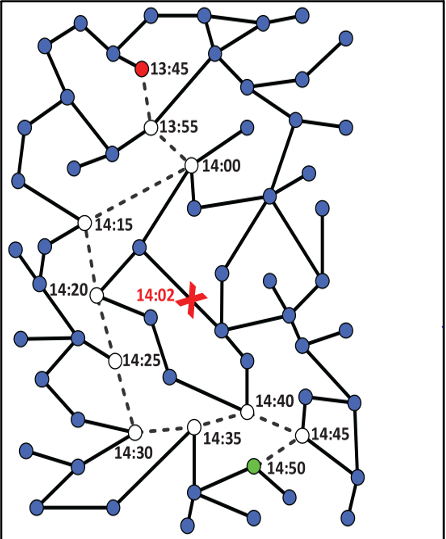
\includegraphics{figures/within_day.png}

}

\caption{\label{fig-within_day}Within-day replanning approach for a
MATSim routing problem.}

\end{figure}

Unfortunately, the problem showcased in Figure~\ref{fig-within_day}
surfaced at times throughout our MATSim simulations. In certain
scenarios, agents preemptively avoided specific road links anticipated
to have incidents, rather than adhering to more realistic behavior
patterns observed on real roads. Typically, drivers maintain their
intended course until directly confronted with congestion or delays, at
which point they may choose to reroute. This variance between the
simulated and actual driver responses to unforeseen road incidents
underscores a key area for enhancement in our simulation model, ensuring
it more accurately reflects realistic driving behavior.

\hypertarget{sec-parameters}{%
\subsection{Initial Parameters}\label{sec-parameters}}

As outlined in \protect\hyperlink{sec-model_imp}{Model Implementation},
we largely derived the initial scoring configuration parameters for our
model from the configuration file used by Kaddoura \& Nagel (2018) in
their MATSim incidents model. Despite the similarities between our
simulations, it is important to note that their model was set in Berlin,
Germany, where average travel patterns, particularly in terms of mode
choice, differ from those in the United States, and more specifically,
Utah. The mode choice parameters in their configuration tended to favor
higher rates of biking and transit use than would likely occur in a
network representing the Utah Wasatch Front. While the absence of
\protect\hyperlink{sec-within-day}{Within-Day Replanning} may have had a
more significant impact, one of the
\protect\hyperlink{sec-next_steps}{Next Steps} for enhancing our model
should certainly involve adjusting the configuration file to more
accurately reflect the authentic travel behaviors of Utah residents.

\hypertarget{sec-next_steps}{%
\section{Next Steps}\label{sec-next_steps}}

Moving forward, enhancing the simulation of IMT response and performance
could be achieved by implementing the adjustments mentioned in the
\protect\hyperlink{sec-limitations}{Limitations}, specifically
concerning the replanning and configuration settings of the MATSim
model. Future steps could also involve exploring additional methods for
simulated analysis of IMT performance measures. Depending on the
specific requirements of UDOT or other transportation agencies, the
simulation could be modified to evaluate optimal IMT starting locations,
hours of operation, or their overall cost-benefit ratio.

Overall, the simulation we developed largely corroborates previous
findings regarding the efficacy of IMT. While it necessitates certain
adjustments to enhance its reliability, it demonstrates potential as a
tool for examining IMT performance in ways that previous studies have
not.

\bookmarksetup{startatroot}

\hypertarget{references}{%
\chapter*{References}\label{references}}
\addcontentsline{toc}{chapter}{References}

\markboth{References}{References}

\hypertarget{refs}{}
\begin{CSLReferences}{1}{0}
\leavevmode\vadjust pre{\hypertarget{ref-bennett2021}{}}%
Bennett, L. S. (2021). \emph{Analysis of benefits of an expansion to
UDOT's incident management program}.

\leavevmode\vadjust pre{\hypertarget{ref-boyles2018}{}}%
Boyles, S. (2018). \emph{Introduction to dynamic traffic assignment}.

\leavevmode\vadjust pre{\hypertarget{ref-day2022}{}}%
Day, C. S. (2022). \emph{Forecasting ride-hailing across multiple model
frameworks}.

\leavevmode\vadjust pre{\hypertarget{ref-dia2006}{}}%
Dia, H., \& Cottman, N. (2006). Evaluation of arterial incident
management impacts using traffic simulation. \emph{Intelligent Transport
Systems, IEE Proceedings}, \emph{153}, 242--252.
\url{https://doi.org/10.1049/ip-its:20055005}

\leavevmode\vadjust pre{\hypertarget{ref-dobler2016}{}}%
Dobler, C., \& Nagel, K. (2016). \emph{Within-day replanning}. {Ubiquity
Press}.

\leavevmode\vadjust pre{\hypertarget{ref-horni2016}{}}%
Horni, A., \& Nagel, K. (2016). \emph{More about conguring MATSim}.
{Ubiquity Press}.

\leavevmode\vadjust pre{\hypertarget{ref-hyer2023}{}}%
Hyer, J. (2023). \emph{Analysis of benefits of UDOT's expanded incident
management team program}.

\leavevmode\vadjust pre{\hypertarget{ref-kaddoura2018}{}}%
Kaddoura, I., \& Nagel, K. (2018). Using real-world traffic incident
data in transport modeling. \emph{Procedia Computer Science},
\emph{130}, 880--885. \url{https://doi.org/10.1016/j.procs.2018.04.084}

\leavevmode\vadjust pre{\hypertarget{ref-kim2012}{}}%
Kim, W., Franz, M., Chang, G.-L., \& University of Maryland (College
Park, Md. ). Dept. of C. and E. E. (2012). \emph{Enhancement of freeway
incident traffic management and resulting benefits.}

\leavevmode\vadjust pre{\hypertarget{ref-lant2021}{}}%
Lant, N. J. (2021). \emph{Estimation and simulation of daily activity
patterns for individuals using wheelchairs}.

\leavevmode\vadjust pre{\hypertarget{ref-li2020}{}}%
Li, J., \& Ferguson, N. (2020). A multi-dimensional rescheduling model
in disrupted transport network using rule-based decision making.
\emph{Procedia Computer Science}, \emph{170}, 90--97.
\url{https://doi.org/10.1016/j.procs.2020.03.012}

\leavevmode\vadjust pre{\hypertarget{ref-lou2011}{}}%
Lou, Y., Yin, Y., \& Lawphongpanich, S. (2011). Freeway service patrol
deployment planning for incident management and congestion mitigation.
\emph{Transportation Research Part C: Emerging Technologies},
\emph{19}(2), 283--295. \url{https://doi.org/10.1016/j.trc.2010.05.014}

\leavevmode\vadjust pre{\hypertarget{ref-nagel2016}{}}%
Nagel, K., Kickhofer, B., Horni, A., \& Charypar, D. (2016). \emph{A
closer look at scoring}. {Ubiquity Press}.

\leavevmode\vadjust pre{\hypertarget{ref-ozbay2013}{}}%
Ozbay, K., Iyigun, C., Baykal-Gursoy, M., \& Xiao, W. (2013).
Probabilistic programming models for traffic incident management
operations planning. \emph{Annals of Operations Research},
\emph{203}(1), 389--406. \url{https://doi.org/10.1007/s10479-012-1174-6}

\leavevmode\vadjust pre{\hypertarget{ref-pal2002}{}}%
Pal, R., \& Sinha, K. C. (2002). {SIMULATION MODEL FOR EVALUATING AND
IMPROVING EFFECTIVENESS OF FREEWAY SERVICE PATROL PROGRAMS}.
\emph{Journal of Transportation Engineering}, \emph{128}(4).

\leavevmode\vadjust pre{\hypertarget{ref-rieser2016}{}}%
Rieser, H., Nagel. (2016). \emph{MATSim data containers}. {Ubiquity
Press}.

\leavevmode\vadjust pre{\hypertarget{ref-schultz2019}{}}%
Schultz, G. G., Saito, M., Eggett, D. L., Bennett, L. S., Hadfield, M.
G., Civil, B. Y. University. Dept. of, \& Environmental Engineering.
(2019). \emph{Analysis of performance measures of traffic incident
management in utah}.

\leavevmode\vadjust pre{\hypertarget{ref-sisiopiku2007}{}}%
Sisiopiku, V. P., Li, X., Mouskos, K. C., Kamga, C., Barrett, C., \&
Abro, A. M. (2007). Dynamic traffic assignment modeling for incident
management. \emph{Transportation Research Record}, \emph{1994}(1),
110--116. \url{https://doi.org/10.3141/1994-15}

\leavevmode\vadjust pre{\hypertarget{ref-skabardonis1998}{}}%
Skabardonis, A., Petty, K., Varaiya, P., \& Bertini, R. (1998).
Evaluation of the freeway service patrol ({FSP}) in los angeles.
\emph{PATH Research Report}.

\leavevmode\vadjust pre{\hypertarget{ref-wirtz2005}{}}%
Wirtz, J. J., Schofer, J. L., \& Schulz, D. F. (2005). Using simulation
to test traffic incident management strategies: {The} benefits of
preplanning. \emph{Transportation Research Record}, \emph{1923}(1),
82--90. \url{https://doi.org/10.1177/0361198105192300109}

\end{CSLReferences}

\cleardoublepage
\phantomsection
\addcontentsline{toc}{part}{Appendices}
\appendix

\hypertarget{event-handlers}{%
\chapter{Event Handlers}\label{event-handlers}}

This is the event handler

\begin{Shaded}
\begin{Highlighting}[]
\KeywordTok{public} \KeywordTok{class}\NormalTok{ Bike }\OperatorTok{\{}
    \BuiltInTok{Integer}\NormalTok{ gears }\OperatorTok{=} \DecValTok{0}\OperatorTok{;}
    \BuiltInTok{String}\NormalTok{ color }\OperatorTok{=} \StringTok{"red"}\OperatorTok{;}
    \BuiltInTok{Double}\NormalTok{ price }\OperatorTok{=} \FloatTok{500.0}\OperatorTok{;}

    \FunctionTok{Bike} \OperatorTok{(}\BuiltInTok{Integer}\NormalTok{ gears}\OperatorTok{,} \BuiltInTok{String}\NormalTok{ color}\OperatorTok{,} \BuiltInTok{Double}\NormalTok{ price}\OperatorTok{)} \OperatorTok{\{}
        \KeywordTok{this}\OperatorTok{.}\FunctionTok{gears} \OperatorTok{=}\NormalTok{ gears}\OperatorTok{;}
        \KeywordTok{this}\OperatorTok{.}\FunctionTok{color} \OperatorTok{=}\NormalTok{ color}\OperatorTok{;}
        \KeywordTok{this}\OperatorTok{.}\FunctionTok{price} \OperatorTok{=}\NormalTok{ price}\OperatorTok{;}
    \OperatorTok{\}}
\OperatorTok{\}}
\end{Highlighting}
\end{Shaded}


\end{document}
